%%%%%%%%%%%%%%%%%%%%%%%%%%%%%%%%%%%%%%%%%%%%%%%%%%%%%%%%%%%%%%%%%%%%%%%%%%%%%%%%%%%%%%%%%%%%%%%%
%
% CS576 Written Question Template
%
% Acknowledgements:
% The original code is written by Prof. James Tompkin (james_tompkin@brown.edu).
% The second version is revised by Prof. Min H. Kim (minhkim@kaist.ac.kr).
%
% This is a LaTeX document. LaTeX is a markup language for producing
% documents. Your task is to fill out this document, then to compile
% it into a PDF document.
%
%
% TO COMPILE:
% > pdflatex thisfile.tex
%
% If you do not have LaTeX and need a LaTeX distribution:
% - Personal laptops (all common OS): www.latex-project.org/get/
% - We recommend latex compiler miktex (https://miktex.org/) for windows,
%   macTex (http://www.tug.org/mactex/) for macOS users.
%   And TeXstudio(http://www.texstudio.org/) for latex editor.
%   You should install both compiler and editor for editing latex.
%   The another option is Overleaf (https://www.overleaf.com/) which is
%   an online latex editor.
%
% If you need help with LaTeX, please come to office hours.
% Or, there is plenty of help online:
% https://en.wikibooks.org/wiki/LaTeX
%
% Good luck!
% Min and the CS576 staff
%
%%%%%%%%%%%%%%%%%%%%%%%%%%%%%%%%%%%%%%%%%%%%%%%%%%%%%%%%%%%%%%%%%%%%%%%%%%%%%%%%%%%%%%%%%%%%%%%%
%
% How to include two graphics on the same line:
%
% \includegraphics[\width=0.49\linewidth]{yourgraphic1.png}
% \includegraphics[\width=0.49\linewidth]{yourgraphic2.png}
%
% How to include equations:
%
% \begin{equation}
% y = mx+c
% \end{equation}
%
%%%%%%%%%%%%%%%%%%%%%%%%%%%%%%%%%%%%%%%%%%%%%%%%%%%%%%%%%%%%%%%%%%%%%%%%%%%%%%%%%%%%%%%%%%%%%%%%

\documentclass[11pt]{article}

\usepackage[english]{babel}
\usepackage[utf8]{inputenc}
\usepackage[colorlinks = true,
            linkcolor = blue,
            urlcolor  = blue]{hyperref}
\usepackage[a4paper,margin=1.5in]{geometry}
\usepackage{stackengine,graphicx}
\usepackage{fancyhdr}
\setlength{\headheight}{15pt}
\usepackage{microtype}
\usepackage{times}
\usepackage{booktabs}

% From https://ctan.org/pkg/matlab-prettifier
\usepackage[numbered,framed]{matlab-prettifier}

\frenchspacing
\setlength{\parindent}{0cm} % Default is 15pt.
\setlength{\parskip}{0.3cm plus1mm minus1mm}

\pagestyle{fancy}
\fancyhf{}
\lhead{Homework Writeup}
\rhead{CS576}
\rfoot{\thepage}

\date{}

\title{\vspace{-1cm}Homework 2 Writeup(20196055 Aashish Waikar)}


\begin{document}
\maketitle
\vspace{-3cm}
\thispagestyle{fancy}

\section*{Instructions}
\begin{itemize}
  \item Describe any interesting decisions you made to write your algorithm.
  \item Show and discuss the results of your algorithm.
  \item Feel free to include code snippets, images, and equations.
  \item There is no page limit.

\end{itemize}

\section*{In the beginning...}

Lorem ipsum dolor sit amet, consectetur adipisicing elit, sed do eiusmod tempor incididunt ut labore et dolore magna aliqua. Ut enim ad minim veniam, quis nostrud exercitation ullamco laboris nisi ut aliquip ex ea commodo consequat. Duis aute irure dolor in reprehenderit in voluptate velit esse cillum dolore eu fugiat nulla pariatur. Excepteur sint occaecat cupidatat non proident, sunt in culpa qui officia deserunt mollit anim id est laborum. See Equation~\ref{eq:one}.

\begin{equation}
a = b + c
\label{eq:one}
\end{equation}

\section*{My code and explanations}

1)My code for HoG feature descriptor in feature\_extraction.py. I have used the existing functions for HoG descriptor and then reshaped h so that the horizontal dimension becomes 36.

\begin{lstlisting}[style=Matlab-editor]
# Your code here. You should also change the return value.
        hog = cv2.HOGDescriptor(win_size,block_size,block_stride,cell_size,nbins,deriv_aperture,win_sigma,histogram_norm_type,l2_hys_threshold,gamma_correction,nlevels)
        h = hog.compute(img)
        
        h=np.reshape(h, (-1,36))
        return h
        #return np.zeros((1500, 36))
\end{lstlisting}

2)My code for SIFT feature descriptor in feature\_extraction.py. I have used the existing functions for SIFT descriptor with grid size 20 x 20.
\begin{lstlisting}[style=Matlab-editor]
# Your code here. You should also change the return value.
        sift = cv2.xfeatures2d.SIFT_create()
        grid = 20
        kp = [cv2.KeyPoint(x, y, grid) for x in range(0, img.shape[0], grid) for y in range(0, img.shape[1], grid)]
        feat = sift.compute(img, kp)       
        return feat[1]
        #return np.zeros((1500, 128))
\end{lstlisting}

3)My code for Kmeans in kmeans\_clustering.py. I have first initialised the vocabulary randomly with vectors from all\_features. Then, in each loop, I first cluster the features using existing vocabulary(assign each feature to the cluster with closest centroid) and then recompute the centroids and update those in the vocabulary. The vocabulary is returned either when the max\_iterations are complete or when the distance b/w centroids in consecutively computed vocabularies becomes less than epsilon.
\begin{lstlisting}[style=Matlab-editor]
# Your code here. You should also change the return value.
    #choosing random centroids
    #print(all_features.shape)

    total_pts=len(all_features[:,0])
    rand_arr=np.random.choice(total_pts, vocab_size, replace=False)
    rand_arr.sort()
    vocab_matrix=np.zeros((vocab_size, all_features.shape[1]))
    class_arr=np.zeros(total_pts)

    # #initialised vocab matrix
    ###########
    for i in range(vocab_size):
        vocab_matrix[i]=all_features[rand_arr[i]]

    #print(vocab_matrix)
    
    for r in range(max_iter):
        #assign each pt to a cluster
        dist_mat = pdist(all_features, vocab_matrix)
        c1=0
        for vec in dist_mat:
            index = np.argmin(vec)
            class_arr[c1]=index
            c1+=1

        #finding new centroids
        class_sum=np.zeros((vocab_size,all_features.shape[1]))
        class_count=np.zeros(vocab_size)
        new_vocab=np.zeros((vocab_size,all_features.shape[1]))

        for i in range(total_pts):
            cur_class=class_arr[i]
            #print(int(cur_class))
            class_sum[int(cur_class)]+=all_features[i]
            class_count[int(cur_class)]+=1

        for i in range(vocab_size):
            if class_count[i]==0:
                new_vocab[i]=vocab_matrix[i]
            else:
                new_vocab[i]=class_sum[i]/class_count[i]
        #print(new_vocab)
        dist_mat1 = pdist(vocab_matrix,new_vocab)

        for c3 in range(vocab_size):
            if dist_mat1[c3][c3]>epsilon :
                break

        vocab_matrix=new_vocab
        #print(vocab_matrix)
        if c3==vocab_size-1:
            break

    return vocab_matrix
\end{lstlisting}

4)My code for PCA in get\_features\_from\_pca.py. I have calculated PCA using the technique of Eigen-value decomposition. First, compute the mean and centre the vectors with respect to it. Then compute the covariance matrix and its eigen value decomposition. Then choose 2 or 3(whichever final dimensionality chosen) eignvectors with the maximum variance and compute reprojections.
\begin{lstlisting}[style=Matlab-editor]
# Your code here. You should also change the return value.

    m=np.mean(vocab.T,axis=1)
    cent_m=vocab-m
    covar=np.cov(cent_m.T)
    val, vec=np.linalg.eig(covar)
    l=val.tolist()
    tup=[l.index(x) for x in sorted(l, reverse=True)[:feat_num]]
    red_vec=np.zeros((vocab.shape[1],feat_num))
    for i in range(feat_num):
        red_vec[:,i]=vec[:,tup[i]]

    P=red_vec.T.dot(cent_m.T)
    return P.T
    #return np.zeros((vocab.shape[0],2))
\end{lstlisting}

5)My code for Bag of words in get\_bag\_of\_words.py. I iterate over all images using a for loop. Then, for each image, I compute features using feature\_extraction.py and then cluster them using the existing trained vocabulary. I compute a new array whose each element represents the frequency of that corresponding vocabulary vector in that image. Finally, these arrays computed in each iteration are stacked with axis = 0 to result in the final matrix which is returned.
\begin{lstlisting}[style=Matlab-editor]
    if feature == 'HoG':
        vocab = np.load('vocab_hog.npy')
    elif feature == 'SIFT':
        vocab = np.load('vocab_sift.npy')

    vocab_size = vocab.shape[0]
    ft_size = vocab.shape[1]

    output_mat=np.zeros((image_paths.shape[0],vocab_size))

    # # Your code here. You should also change the return value.
    i=0
    for path in image_paths:
        #dealing with one image
        img = cv2.imread(path)[:, :, ::-1]
        #total_ft*featurevect_length
        features = feature_extraction(img, feature)
        distance_mat = pdist(features,vocab)
        for vec in distance_mat:
            index = np.argmin(vec)
            output_mat[i][index]+=1
        output_mat[i] = output_mat[i] / linalg.norm(output_mat[i])
        i=i+1

    return output_mat
\end{lstlisting}

6)My code for Spatial Pyramid in get\_spatial\_pyramid\_feats.py. Here, the change is that in each iteration, I compute the histograms for each image and its set of subimages according to max\_level. All these histograms are appended to result in 1 single array for each iteration. This array represents the features for the current image(we hope that it has some spatial information now). These arrays are stacked vertically to result in the final matrix.
\begin{lstlisting}[style=Matlab-editor]
    # Your code here. You should also change the return value.
    ft_size = vocab.shape[1]

    output_mat=np.zeros((1,vocab_size))

    # # Your code here. You should also change the return value.
    i=0
    for path in image_paths:
        #dealing with one image
        img = cv2.imread(path)[:, :, ::-1]
        hor = img.shape[1]
        ver = img.shape[0]
        
        f_image_mat=np.zeros((1,1))
        for l in range(max_level+1):
            hstep = math.floor(hor/(2**l))
            vstep = math.floor(ver/(2**l))
            x, y = 0, 0
            for c1 in range(1,2**l + 1):
                x = 0
                for c2 in range(1, 2**l + 1):                
                    features = feature_extraction(img[y:y+vstep, x:x+hstep], feature)                
                    #print("type:",desc is None, "x:",x,"y:",y, "desc_size:",desc is None)
                    distance_mat = pdist(features,vocab)
                    row = np.zeros(vocab_size)
                    for vec in distance_mat:
                        index = np.argmin(vec)
                        row[index]+=1
                    weight = 2**(l-max_level)
                    f_row_mat = np.zeros((1,vocab_size))
                    f_row_mat[0] = weight*row
                    f_image_mat = np.append(f_image_mat, f_row_mat, axis=1)

                    x = x + hstep
                y = y + vstep
        if i==0:
            output_mat = np.append(output_mat, f_image_mat[:,1:], axis=1)
            output_mat = output_mat[:,vocab_size:]
        else:
            output_mat = np.append(output_mat, f_image_mat[:,1:], axis=0)
        i+=1
    #output_mat = output_mat[1:,:]
    output_mat = (1 / 3) * (4 ^ (max_level + 1) - 1) * output_mat

    #print(output_mat)
    return output_mat
\end{lstlisting}

7)My code for svm in svm\_classify.py. Here, I loop over all the categories and then train svm classifier for the current category vs all other othegories. I initialise the classifier with kernel=kernel\_type which is either 'linear' or 'rbf'  and use C=0.025. I varied C and chose this as it gave good performance. Then, I train the svm with training data and compute the confidence score using classifier.decision\_function(). Finally, the category which gets the highest confidence for the image is the predicted label.
\begin{lstlisting}[style=Matlab-editor]
    # Your code here. You should also change the return value.

    pred_labels = train_labels
    cfd_matrix = np.zeros((test_image_feats.shape[0], len(categories)))
    i=0

    for categ in categories:
        new_train_labels1 = np.zeros(len(train_labels))
        new_train_labels1 = np.where(train_labels==categ,1,new_train_labels1)
        classifier = svm.SVC(random_state=0,C=0.025,kernel=kernel_type)
        classifier.fit(train_image_feats, new_train_labels1)
        cfd_arr = classifier.decision_function(test_image_feats)
        cfd_matrix[:,i] = cfd_arr
        i+=1

    j=0
    for vec in cfd_matrix:
        index = np.argmax(vec)
        pred_labels[j] = categories[index]
        j+=1


    return pred_labels
\end{lstlisting}

\section*{PCA result}

\begin{enumerate}
    %\item Result 1 was a total failure, because...
    \item Result 1(HOG) (left)
    \item Result 2(SIFT) (right)
\end{enumerate}

\begin{figure}[h]
    \centering
    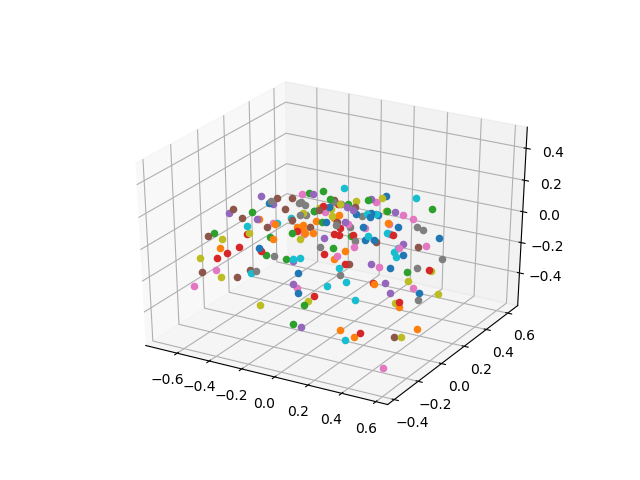
\includegraphics[width=5cm]{hog.png}
    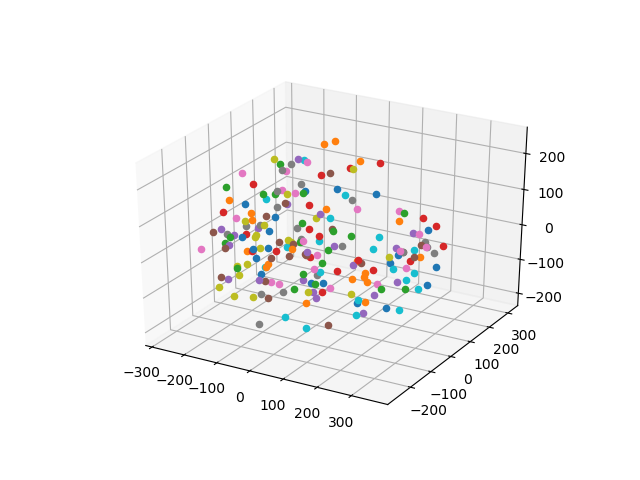
\includegraphics[width=5cm]{sift.png}
    \caption{\emph{Left:} HOG \emph{Right:} SIFT}
    \label{fig:result1}
\end{figure}

Recognition accuracy of SIFT vs HOG(linear kernel and spatial pyramid)~\ref{tab:table1}.

\begin{table}[h]
    \centering
    \begin{tabular}{lr}
        \toprule
        Condition & accuracy \\
        \midrule
        SIFT & 0.725 \\
        HOG & 0.691 \\
        \bottomrule
    \end{tabular}
    \caption{SIFT vs HOG}
    \label{tab:table1}
\end{table}

Recognition accuracy of SIFT vs HOG(linear kernel and bag of words)~\ref{tab:table2}.

\begin{table}[h]
    \centering
    \begin{tabular}{lr}
        \toprule
        Condition & accuracy \\
        \midrule
        SIFT & 0.635 \\
        HOG & 0.559 \\
        \bottomrule
    \end{tabular}
    \caption{SIFT vs HOG}
    \label{tab:table2}
\end{table}

Recognition accuracy of linear vs rbf(using sift and bag of words with spatial pyramid)~\ref{tab:table3}.

\begin{table}[h]
    \centering
    \begin{tabular}{lr}
        \toprule
        Condition & accuracy \\
        \midrule
        linear & 0.725\\
        rbf & 0.707\\
        \bottomrule
    \end{tabular}
    \caption{linear vs rbf}
    \label{tab:table3}
\end{table}

Recognition accuracy of bag of words without and with spatial pyramid (using sift and linear kernel)~\ref{tab:table4}.

\begin{table}[h]
    \centering
    \begin{tabular}{lr}
        \toprule
        Condition & accuracy\\
        \midrule
        without\_spatial\_pyramid & 0.635\\
        with\_spatial\_pyramid & 0.725\\
        \bottomrule
    \end{tabular}
    \caption{with andd without spatial pyramid}
    \label{tab:table4}
\end{table}

\section*{Confusion matrix(for spatial pyramid with sift features and rbf kernel)}

\begin{enumerate}
    %\item Result 1 was a total failure, because...
    \item Confusion matrix with accuracy 0.707
\end{enumerate}

\begin{figure}[h]
    \centering
    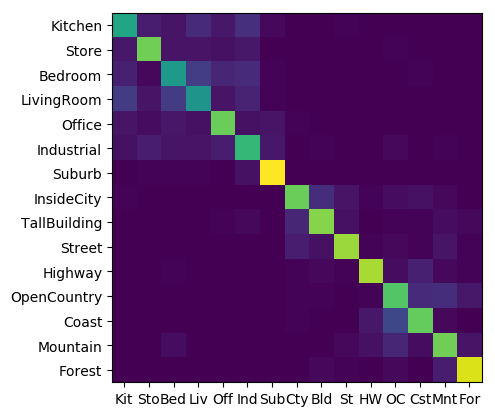
\includegraphics[width=10cm]{confusion_matrix.png}
    %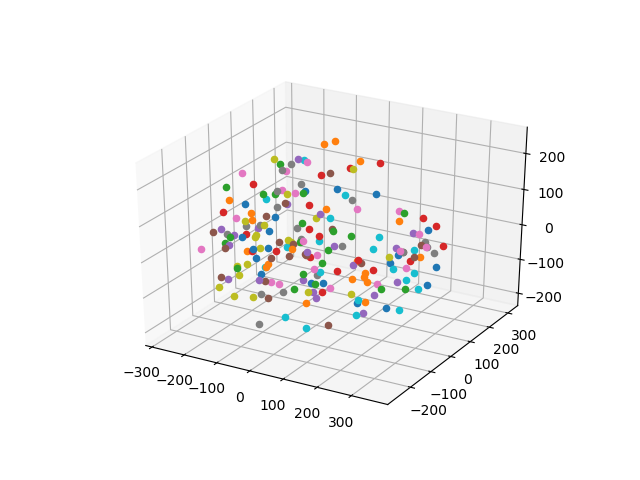
\includegraphics[width=5cm]{sift.png}
    %\caption{\emph{Left:} HOG \emph{Right:} SIFT}
    %\label{fig:result1}
\end{figure}

The result in stored in file index.html

\end{document} 